\section{Perspectiva dentro del IDU}

\begin{figure}[h]
 \centering6
 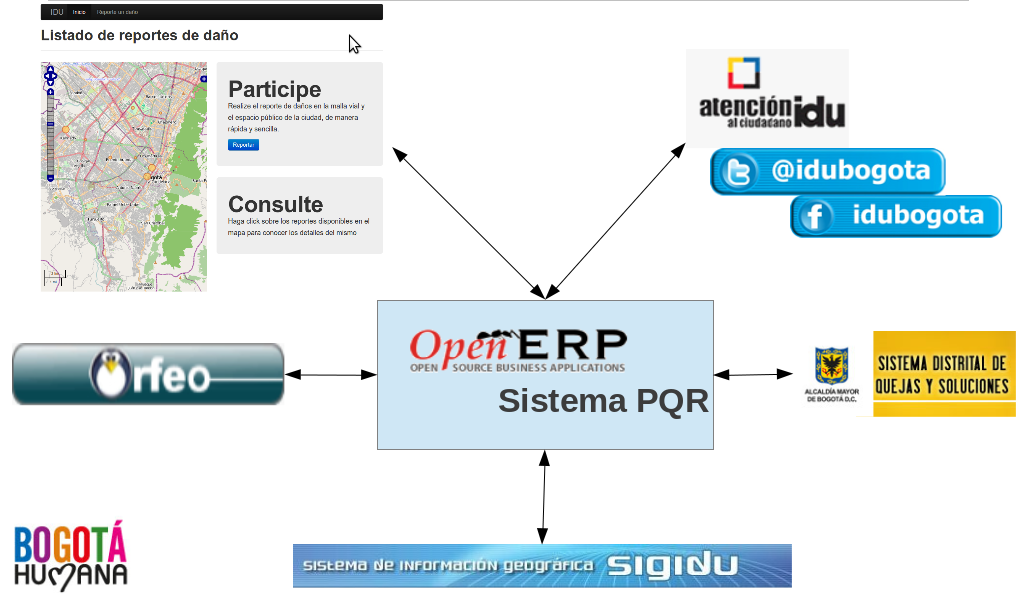
\includegraphics[width=17cm,height=9.5cm]{./Imagenes/slidesistemacompleto.png}
 % Login.png: 1289x610 pixel, 96dpi, 34.10x16.14 cm, bb=0 0 967 457
 \caption{Perspectiva actual del sistema OpenErp dentro del IDU}
 \label{fig:slidesistemacompleto}
\end{figure}

Al interior del IDU el módulo se integra a los demás sistemas de información como tal como se ve en la figura \ref{fig:slidesistemacompleto}. OpenErp consolida la 
información de todas las PQR que ingresan al instituto. A su vez cuenta con los mecanismos para comunicarse con los otros sistemas de información 
relacionados: Sistema de Información Geográfico del IDU (SIGIDU), Sistema de Gestión Documental (Orfeo GPL), Sistema Distrital de 
Quejas y Soluciones (SDQS). \\

Las PQR se tramitan de la siguiente manera: Se registran en OpenErp, allí son gestionadas por la Oficina de atención al ciudadano,
si no se cuenta con una respuesta inmediata, pasan a la dependencia relacionada de la organización a través del
sistema de Gestion Documental Orfeo, OpenErp espera la respuesta y conserva el número de radicación de Orfeo. Los casos y los documentos, son copiados también 
a SDQS, lo cual es necesario para cumplir la normativa distrital.\\

El ciudadano dispone de una herramienta para registrar su PQR desde el portal Web Institucional,se trata del portal de Huecos,
desde ahí se diligencia un formulario con toda la información relacionada a los daños de la malla vial, se hace una clasificación y se ubica el 
punto en el mapa de la ciudad. El reporte es almacenado en Openerp y luego tramitado.\\

Si un ciudadano llega personalmente a las instalaciones del IDU y radica un documento, este es digitalizado, ingresa al sistema Orfeo, si el 
documento se cataloga como una PQR, pasa automáticamente a OpenErp para que sea tramitado.\\

Si el ciudadano ingresa a la página de Internet de SDQS y crea una petición, esta es remitida al IDU por servicios Web, ingresa directamente a OpenErp, 
y allí se inicia el trámite correspondiente.\\




